
\documentclass[a4paper,11pt]{article}%,twocolumn
%% packages

\usepackage{blindtext} % needed for creating dummy text passages
%\usepackage{ngerman} % needed for German default language
\usepackage{amsmath} % needed for command eqref
\usepackage{amssymb} % needed for math fonts
\usepackage[colorlinks=true,breaklinks]{hyperref} % needed for creating hyperlinks in the document, the option colorlinks=true gets rid of the awful boxes, breaklinks breaks lonkg links (list of figures), and ngerman sets everything for german as default hyperlinks language
\usepackage[hyphenbreaks]{breakurl} % ben�tigt f�r das Brechen von URLs in Literaturreferenzen, hyphenbreaks auch bei links, die �ber eine Seite gehen (mit hyphenation).
\usepackage{xcolor}
\definecolor{c1}{rgb}{0,0,1} % blue
\definecolor{c2}{rgb}{0,0.3,0.9} % light blue
\definecolor{c3}{rgb}{0.3,0,0.9} % red blue
\hypersetup{
    linkcolor={c1}, % internal links
    citecolor={c2}, % citations
    urlcolor={c3} % external links/urls
}
%\usepackage{cite} % needed for cite
\usepackage[square,authoryear]{natbib} % needed for cite and abbrvnat bibliography style
\usepackage[nottoc]{tocbibind} % needed for displaying bibliography and other in the table of contents
\usepackage{graphicx} % needed for \includegraphics 
\usepackage{longtable} % needed for long tables over pages
\usepackage{bigstrut} % needed for the command \bigstrut
\usepackage{enumerate} % needed for some options in enumerate
%\usepackage{todonotes} % needed for todos
\usepackage{makeidx} % needed for creating an index
\makeindex
\usepackage{gensymb}
\usepackage{url}
\usepackage{psfrag}
\usepackage{multirow}
\usepackage{subfigure}
%% page settings

\usepackage[top=20mm, bottom=20mm,left=15mm,right=15mm]{geometry} % needed for page border settings
\parindent=0mm % for space of first line of new text block
\sloppy % for writing with hyphenless justification (tries to)
\hyphenation{} % use hyphenation of tolerance parametershttp://www.jr-x.de/publikationen/latex/tipps/zeilenumbruch.html
\hyphenpenalty=10000
\exhyphenpenalty=10000
\usepackage{fancyhdr} % needed for head and foot options
%% my macros

%% Text fomats
\newcommand{\tbi}[1]{\textbf{\textit{#1}}}

%% Math fonts
\newcommand{\bbA}{\mathbb{A}}
\newcommand{\bbB}{\mathbb{B}}
\newcommand{\bbC}{\mathbb{C}}
\newcommand{\bbD}{\mathbb{D}}
\newcommand{\bbE}{\mathbb{E}}
\newcommand{\bbF}{\mathbb{F}}
\newcommand{\bbG}{\mathbb{G}}
\newcommand{\bbH}{\mathbb{H}}
\newcommand{\bbI}{\mathbb{I}}
\newcommand{\bbJ}{\mathbb{J}}
\newcommand{\bbK}{\mathbb{K}}
\newcommand{\bbL}{\mathbb{L}}
\newcommand{\bbM}{\mathbb{M}}
\newcommand{\bbN}{\mathbb{N}}
\newcommand{\bbO}{\mathbb{O}}
\newcommand{\bbP}{\mathbb{P}}
\newcommand{\bbQ}{\mathbb{Q}}
\newcommand{\bbR}{\mathbb{R}}
\newcommand{\bbS}{\mathbb{S}}
\newcommand{\bbT}{\mathbb{T}}
\newcommand{\bbU}{\mathbb{U}}
\newcommand{\bbV}{\mathbb{V}}
\newcommand{\bbW}{\mathbb{W}}
\newcommand{\bbX}{\mathbb{X}}
\newcommand{\bbY}{\mathbb{Y}}
\newcommand{\bbZ}{\mathbb{Z}}
\usepackage[ framed, numbered]{matlab-prettifier}%framed,%
\usepackage{listings}
\usepackage{physics}
\usepackage{pdfpages}
\usepackage[toc,page]{appendix}
\usepackage{float}
\usepackage{hyperref}

\newenvironment{qanda}{\setlength{\parindent}{0pt}}{\bigskip}
\newcommand{\Q}{\bigskip\bfseries Q: }
\newcommand{\A}{\par\textbf{Answer: } \normalfont}

\begin{document}
\begin{titlepage}
\center % Center everything on the page

%-------------------------------------------------------------------------------------
%	HEADING SECTIONS
%------------------------------------------------------------------------------------
\textbf{\large Department of Electrical and Computer Engineering}\\[0.5cm]
\textbf{\Large University of Colorado at Boulder}\\[1cm]
\textbf{\large ECEN5623 - Real Time Embedded Systems }\\[2cm]

\includegraphics[width=0.3\textwidth]{figures/cu}\\[2cm]

	
%-------------------------------------------------------------------------------------
%	TITLE SECTION
%------------------------------------------------------------------------------------
\textbf{\Huge Exercise 5 }\\[0.2cm]



%----------------------------------------------------------------------------------------
%	MEMBERS SECTION
%----------------------------------------------------------------------------------------


\vfill

\textbf{\large Submitted by}\\[0.5cm]

{\large Parth | Jithedra}\\[0.5cm]	

%----------------------------------------------------------------------------------------
%	DATE SECTION
%----------------------------------------------------------------------------------------

\textbf{\large Submitted on}
\textbf{\Large \today} % Date, change the \today to a set date if you want to be precise

%----------------------------------------------------------------------------------------

\vfill % Fill the rest of the page with whitespace

\end{titlepage}


\pagebreak

\tableofcontents
\listoffigures
\listoftables
\vfill
\begin{center}
	\textbf{\textit{*PDF is clickable}}
\end{center}

\pagebreak



\begin{qanda}

	\section{Question 1}
	\Q  Develop an example of a 32-bit Hamming encoded word (39 bits total) and show a correctable SBE
	scenario. Show the data word in a table like Figure 5.6 in the book.
	\addcontentsline{toc}{subsection}{Answer}
	\A
	For example, let's take a 32-bit integer:
	\begin{itemize}
	\item Binary: \texttt{0b10110011010100101100110101001011}
	\item Hexadecimal: \texttt{0xB352CD4B}
	\item Decimal: \texttt{3008548171}
	\end{itemize}
	
	\begin{verbatim}
	_ _ _ 1 _ 1 0 1 _ 0 0 1 0 1 0 1 _ 1 0 0 1 1 0 1 0 0 1 0 1 0 1 1 _ 0 0 1 1 0 1
	\end{verbatim}
	I can't fit image in pdf but there is excel sheet in the same zip folder

	\begin{figure}[H]
		\centering
		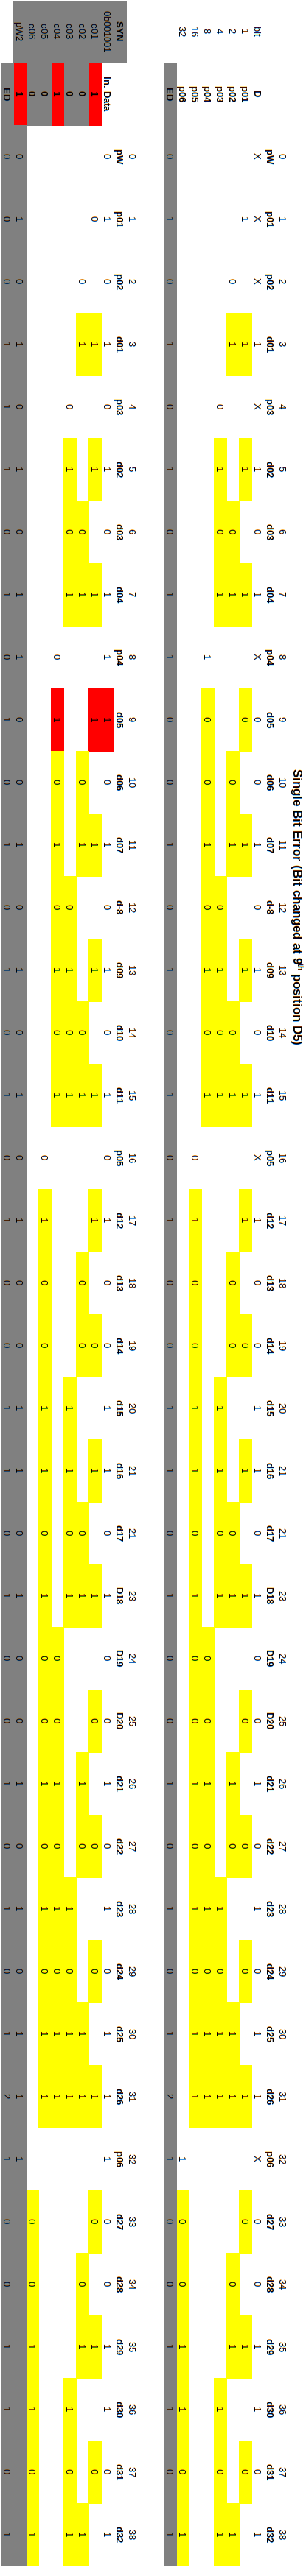
\includegraphics[scale=0.6]{figures/q1.png}
	\end{figure}
	
	With that number, we need to calculate all the parities:
	
	\begin{align*}
p1 &= \text{XOR}(d1, d2, d4, d5, d7, d9, d11, d12, d14, d16, d18, d20, d22, d24, d26, d27, d29, d31) \\
p2 &= \text{XOR}(d1, d3, d4, d6, d7, d10, d11, d13, d14, d17, d18, d21, d22, d25, d26, d28, d29, d32) \\
p3 &= \text{XOR}(d2, d3, d4, d8, d9, d10, d11, d15, d16, d17, d18, d23, d24, d25, d26, d30, d31, d32) \\
p4 &= \text{XOR}(d5, d6, d7, d8, d9, d10, d11, d19, d20, d21, d22, d23, d24, d25, d26) \\
p5 &= \text{XOR}(d12, d13, d14, d15, d16, d17, d18, d19, d20, d21, d22, d23, d24, d25, d26) \\
p6 &= \text{XOR}(d27, d28, d29, d30, d31, d32)
	\end{align*}

	Here are the parity equations with the actual data bit values and the calculated parity bits:
	Given the data bits:

	\begin{verbatim}
	_ _ _ 1 _ 1 0 1 _ 0 0 1 0 1 0 1 _ 1 0 0 1 1 0 1 0 0 1 0 1 0 1 1 _ 0 0 1 1 0 1
	\end{verbatim}
	
	The parity bits can be calculated as follows:
	
	\begin{align*}
p1 &= \text{XOR}(d1, d2, d4, d5, d7, d9, d11, d12, d14, d16, d18, d20, d22, d24, d26, d27, d29, d31) \\
&= \text{XOR}(1, 1, 1, 0, 1, 1, 1, 1, 0, 1, 1, 0, 0, 0, 1, 0, 1, 0) \\
&= 1 \\
p2 &= \text{XOR}(d1, d3, d4, d6, d7, d10, d11, d13, d14, d17, d18, d21, d22, d25, d26, d28, d29, d32) \\
&= \text{XOR}(1, 0, 1, 0, 1, 0, 1, 0, 0, 0, 1, 1, 0, 1, 1, 0, 1, 1) \\
&= 0 \\
p3 &= \text{XOR}(d2, d3, d4, d8, d9, d10, d11, d15, d16, d17, d18, d23, d24, d25, d26, d30, d31, d32) \\
&= \text{XOR}(1, 0, 1, 0, 1, 0, 1, 1, 1, 0, 1, 1, 0, 1, 1, 1, 0, 1) \\
&= 0 \\
p4 &= \text{XOR}(d5, d6, d7, d8, d9, d10, d11, d19, d20, d21, d22, d23, d24, d25, d26) \\
&= \text{XOR}(0, 0, 1, 0, 1, 0, 1, 0, 0, 1, 0, 1, 0, 1, 1) \\
&= 1 \\
p5 &= \text{XOR}(d12, d13, d14, d15, d16, d17, d18, d19, d20, d21, d22, d23, d24, d25, d26) \\
&= \text{XOR}(1, 0, 0, 1, 1, 0, 1, 0, 0, 1, 0, 1, 0, 1, 1) \\
&= 0 \\
p6 &= \text{XOR}(d27, d28, d29, d30, d31, d32) \\
&= \text{XOR}(0, 0, 1, 1, 0, 1) \\
&= 1
	\end{align*}
	
	The whole word parity bit (pW) can be calculated by XORing all the data bits and parity bits:
	
	\begin{align*}
pW &= \text{XOR}(p1, p2, d1, p3, d2, d3, d4, p4, d5, d6, d7, d8, d9, d10, d11, \\
&\quad p5, d12, d13, d14, d15, d16, d17, d18, d19, d20, d21, d22, d23, d24, d25, d26, \\
&\quad p6, d27, d28, d29, d30, d31, d32) \\
&= \text{XOR}(1, 0, 0, 1, 1, 0, 1, 0, 0, 0, 1, 0, 1, 0, 1, 1, 1, 0, 0, 1, 1, 0, 1, 0, 0, 1, 0, 1, 1, 0, 1, 1, 0, 0, 1, 1, 0, 1) \\
&= 0
	\end{align*}
	
	Therefore, the parity bits and the whole word parity bit for the given data bits are:


	\begin{verbatim}
pW p1 p2 d1 p3 d2 d3 d4 p4 d5 d6 d7 d8 d9 d10 d11
0  1  0  1  0  1  0  1  1  0  0  1  0  1   0   1

p5 d12 d13 d14 d15 d16 d17 d18 d19 d20 d21 d22 d23 d24 d25 d26
0   1   0   0   1   1   0   1   0   0   1   0   1   1   0

p6 d27 d28 d29 d30 d31 d32
1   0   0   1   1   0   1
		\end{verbatim}

	and we are switching one bit at bit position d5(9th bit) so bit position d5(9th bit) is 0 in out case and we are flipping that 
	so we would get

	\begin{itemize}
	\item Binary: \texttt{0b10110011010100101100110101011011}
	\item Hexadecimal: \texttt{0xB352CD5B}
	\item Decimal: \texttt{3008548187}
	\end{itemize}
	
	
	
	\begin{verbatim}
__ __ __ 1 __ 1 0 1 __ 1 0 1 0 1 0 1 __ 1 0 0 1 1 0 1 0 0 1 0 1 0 1 1 __ 0 0 1 1 1 1
\end{verbatim}
		
\begin{align*}
p1 &= \text{XOR}(d1, d2, d4, d5, d7, d9, d11, d12, d14, d16, d18, d20, d22, d24, d26, d27, d29, d31) \\
&= \text{XOR}(1, 1, 1, 1, 1, 1, 1, 1, 0, 1, 1, 0, 0, 0, 1, 0, 1, 0) \\
&= 0 \\
p2 &= \text{XOR}(d1, d3, d4, d6, d7, d10, d11, d13, d14, d17, d18, d21, d22, d25, d26, d28, d29, d32) \\
&= \text{XOR}(1, 0, 1, 0, 1, 0, 1, 0, 0, 0, 1, 1, 0, 1, 1, 0, 1, 1) \\
&= 0 \\
p3 &= \text{XOR}(d2, d3, d4, d8, d9, d10, d11, d15, d16, d17, d18, d23, d24, d25, d26, d30, d31, d32) \\
&= \text{XOR}(1, 0, 1, 0, 1, 0, 1, 1, 1, 0, 1, 1, 0, 1, 1, 1, 0, 1) \\
&= 0 \\
p4 &= \text{XOR}(d5, d6, d7, d8, d9, d10, d11, d19, d20, d21, d22, d23, d24, d25, d26) \\
&= \text{XOR}(1, 0, 1, 0, 1, 0, 1, 0, 0, 1, 0, 1, 0, 1, 1) \\
&= 0 \\
p5 &= \text{XOR}(d12, d13, d14, d15, d16, d17, d18, d19, d20, d21, d22, d23, d24, d25, d26) \\
&= \text{XOR}(1, 0, 0, 1, 1, 0, 1, 0, 0, 1, 0, 1, 0, 1, 1) \\
&= 0 \\
p6 &= \text{XOR}(d27, d28, d29, d30, d31, d32) \\
&= \text{XOR}(0, 0, 1, 1, 0, 1) \\
&= 1
\end{align*}
		
		The whole word parity bit (pW) can be calculated by XORing all the data bits and parity bits:
		
		\begin{align*}
		pW &= \text{XOR}(p1, p2, d1, p3, d2, d3, d4, p4, d5, d6, d7, d8, d9, d10, d11, \\
		&\quad p5, d12, d13, d14, d15, d16, d17, d18, d19, d20, d21, d22, d23, d24, d25, d26, \\
		&\quad p6, d27, d28, d29, d30, d31, d32) \\
		&= \text{XOR}(0, 0, 1, 0, 1, 0, 1, 1, 1, 1, 1, 1, 1, 0, 1, 1, 1, 0, 0, 1, 1, 0, 1, 0, 0, 1, 0, 1, 1, 0, 1, 0, 0, 0, 1, 1, 1, 1) \\
		&= 1
		\end{align*}
		
		Therefore, the output with the parity bits for the modified data with the flipped bit at position 4 is:
		
\begin{verbatim}
pW p1 p2 d1 p3 d2 d3 d4 p4 d5 d6 d7 d8 d9 d10 d11 p5 d12 d13 d14 d15
0  0  0  1  0  1  0  1  0  1  1  1  1  1   0   1  1   1   0   0   1

d16 d17 d18 d19 d20 d21 d22 d23 d24 d25 d26 p6 d27 d28 d29 d30 d31 d32
1   0   1   0   0   1   0   1   1   0   1  1   0   0   1   1   1   1
\end{verbatim}

Comparing the recalculated parity bits with the received parity bits:

p1' != p1 (mismatches the received p1) => c1 = 1
p2' == p2 (matches the received p2) => c2 = 0
p3' == p3 (matches the received p3) => c3 = 0
p4' != p4 (mismatches the received p4) => c4 = 1
p5' == p5 (matches the received p5) => 0
p6' == p6 (matches the received p6) => 0


and pW' != pW that means there is single bit error and we can correct it

arranging c1, c2, c3, c4, c5, c6 will give as 0b001001 which is basically 9 in binary so 9th bit(d5) is wrong in out case D5 is wrong. which proves the point
	\pagebreak
	\section{Question 2}
	\Q   For the foregoing problem, now show an uncorrectable MBE scenario.
	\addcontentsline{toc}{subsection}{Answer}
	\A

	Original Data
	\begin{itemize}
	\item Binary: \texttt{0b10110011010100101100110101001011}
	\item Hexadecimal: \texttt{0xB352CD4B}
	\item Decimal: \texttt{3008548171}
	\end{itemize}
	
\begin{verbatim}
pW p1 p2 d1 p3 d2 d3 d4 p4 d5 d6 d7 d8 d9 d10 d11
0  1  0  1  0  1  0  1  1  0  0  1  0  1   0   1

p5 d12 d13 d14 d15 d16 d17 d18 d19 d20 d21 d22 d23 d24 d25 d26
0   1   0   0   1   1   0   1   0   0   1   0   1   1   0

p6 d27 d28 d29 d30 d31 d32
1   0   0   1   1   0   1
\end{verbatim}

	Data with two bit errors at positions d5 and d6:
	\begin{itemize}
	\item Binary: \texttt{0b10110011010100101100110101001011}
	\item Hexadecimal: \texttt{0xD2ACC5B3}
	\item Decimal: \texttt{3534536627}
	\end{itemize}
	

\begin{verbatim}
	pW p1 p2 d1 p3 d2 d3 d4 p4 d5 d6 d7 d8 d9 d10 d11
	0  1  0  1  0  1  0  1  1  1  1  1  0  1   0   1

	p5 d12 d13 d14 d15 d16 d17 d18 d19 d20 d21 d22 d23 d24 d25 d26
	0   1   0   0   1   1   0   1   0   0   1   0   1   1   0

	p6 d27 d28 d29 d30 d31 d32
	1   0   0   1   1   0   1
\end{verbatim}
I can't fit image in pdf but there is excel sheet in the same zip folder
\begin{figure}[H]
	\centering
	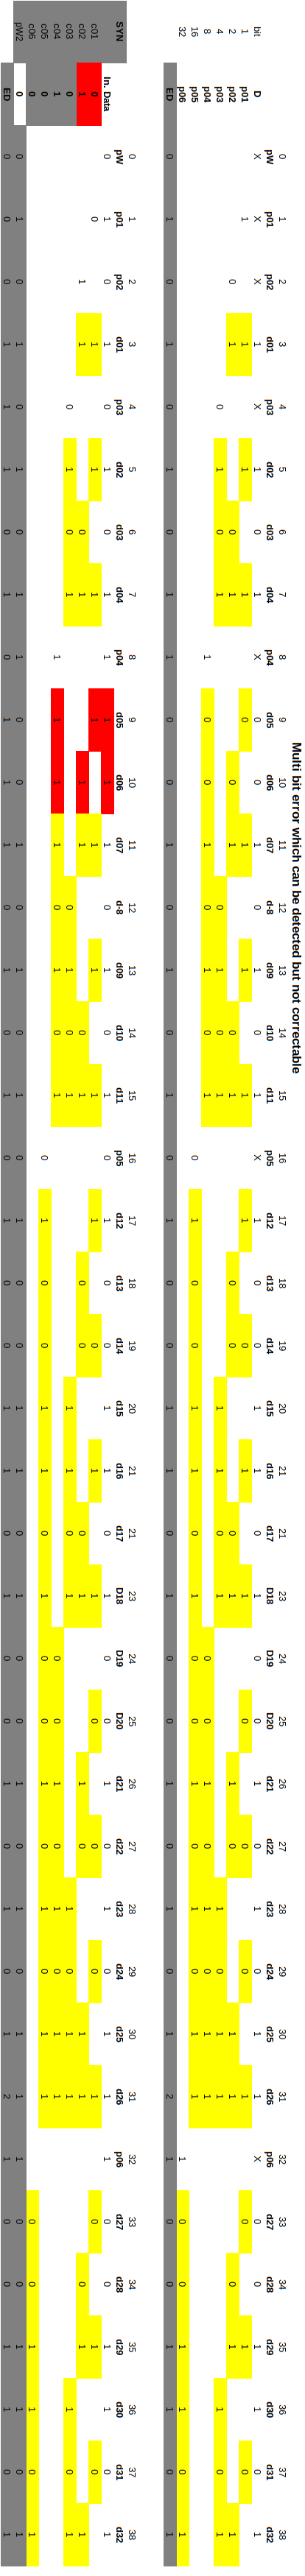
\includegraphics[scale=0.6]{figures/q2.png}
\end{figure}
	
	With that number, we need to calculate all the parities:
	
	\begin{align*}
p1 &= \text{XOR}(d1, d2, d4, d5, d7, d9, d11, d12, d14, d16, d18, d20, d22, d24, d26, d27, d29, d31) \\
p2 &= \text{XOR}(d1, d3, d4, d6, d7, d10, d11, d13, d14, d17, d18, d21, d22, d25, d26, d28, d29, d32) \\
p3 &= \text{XOR}(d2, d3, d4, d8, d9, d10, d11, d15, d16, d17, d18, d23, d24, d25, d26, d30, d31, d32) \\
p4 &= \text{XOR}(d5, d6, d7, d8, d9, d10, d11, d19, d20, d21, d22, d23, d24, d25, d26) \\
p5 &= \text{XOR}(d12, d13, d14, d15, d16, d17, d18, d19, d20, d21, d22, d23, d24, d25, d26) \\
p6 &= \text{XOR}(d27, d28, d29, d30, d31, d32)
	\end{align*}


	
	The parity bits can be calculated as follows:
	
	\begin{align*}
p1 &= \text{XOR}(d1, d2, d4, d5, d7, d9, d11, d12, d14, d16, d18, d20, d22, d24, d26, d27, d29, d31) \\
&= \text{XOR}(1, 1, 1, 0, 1, 1, 1, 1, 0, 1, 1, 0, 0, 0, 1, 0, 1, 0) \\
&= 0 \\
p2 &= \text{XOR}(d1, d3, d4, d6, d7, d10, d11, d13, d14, d17, d18, d21, d22, d25, d26, d28, d29, d32) \\
&= \text{XOR}(1, 0, 1, 0, 1, 1, 1, 0, 0, 0, 1, 1, 0, 1, 1, 0, 1, 1) \\
&= 1 \\
p3 &= \text{XOR}(d2, d3, d4, d8, d9, d10, d11, d15, d16, d17, d18, d23, d24, d25, d26, d30, d31, d32) \\
&= \text{XOR}(1, 0, 1, 0, 1, 0, 1, 1, 1, 0, 1, 1, 0, 1, 1, 1, 0, 1) \\
&= 0 \\
p4 &= \text{XOR}(d5, d6, d7, d8, d9, d10, d11, d19, d20, d21, d22, d23, d24, d25, d26) \\
&= \text{XOR}(1, 1, 1, 0, 1, 0, 1, 0, 0, 1, 0, 1, 0, 1, 1) \\
&= 0 \\
p5 &= \text{XOR}(d12, d13, d14, d15, d16, d17, d18, d19, d20, d21, d22, d23, d24, d25, d26) \\
&= \text{XOR}(1, 0, 0, 1, 1, 0, 1, 0, 0, 1, 0, 1, 0, 1, 1) \\
&= 0 \\
p6 &= \text{XOR}(d27, d28, d29, d30, d31, d32) \\
&= \text{XOR}(0, 0, 1, 1, 0, 1) \\
&= 1
	\end{align*}
	
	The whole word parity bit (pW) can be calculated by XORing all the data bits and parity bits:
	
	\begin{align*}
pW &= \text{XOR}(p1, p2, d1, p3, d2, d3, d4, p4, d5, d6, d7, d8, d9, d10, d11, \\
&\quad p5, d12, d13, d14, d15, d16, d17, d18, d19, d20, d21, d22, d23, d24, d25, d26, \\
&\quad p6, d27, d28, d29, d30, d31, d32) \\
&= \text{XOR}(1, 0, 0, 1, 1, 0, 1, 0, 0, 0, 1, 0, 1, 0, 1, 1, 1, 0, 0, 1, 1, 0, 1, 0, 0, 1, 0, 1, 1, 0, 1, 1, 0, 0, 1, 1, 0, 1) \\
&= 1
	\end{align*}
	
	Therefore, the parity bits and the whole word parity bit for the given data bits are:


	\begin{verbatim}
pW p1 p2 d1 p3 d2 d3 d4 p4 d5 d6 d7 d8 d9 d10 d11
1  0  1  1  0  1  0  1  0  1  1  1  0  1   0   1

p5 d12 d13 d14 d15 d16 d17 d18 d19 d20 d21 d22 d23 d24 d25 d26
0   1   0   0   1   1   0   1   0   0   1   0   1   1   0

p6 d27 d28 d29 d30 d31 d32
1   0   0   1   1   0   1
		\end{verbatim}

Comparing the recalculated parity bits with the received parity bits:

p1' != p1 (mismatches the received p1) => c1 = 1
p2' != p2 (matches the received p2) => c2 = 0
p3' == p3 (matches the received p3) => c3 = 0
p4' == p4 (mismatches the received p4) => c4 = 1
p5' == p5 (matches the received p5) => 0
p6' == p6 (matches the received p6) => 0

and parity word pW' == pW so there is multibit error but we can't correct that

	\pagebreak
	\section{Question 3}
	\Q  For the following Nand flash block update history for 2 sectors that contain 4 blocks each (e.g. 16K
	sectors, with 4K blocks), fill in the missing WRITE operations as needed and compute write-
	amplification.\\
	\begin{figure}[H]
		\centering
		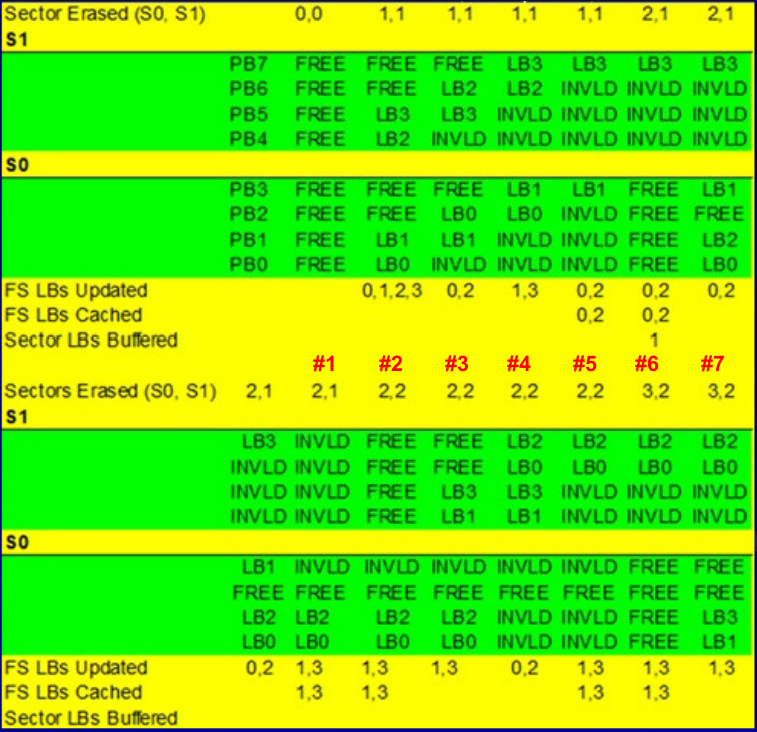
\includegraphics[scale=0.6]{figures/q3.png}
	\end{figure}
	\#1 - All blocks FREE\\
	\#2 - Erase S0 \& S1, WRITE \_\_\_\_\_\_\_\_\_\_\_\_\_\_\_\_\_\_\_\_\_\_\_\_\_\_\_\_\\
	\#3 - Read LB 0, 2, Modify, WRITE \_\_\_\_\_\_\_\_\_\_\_\_\_\_\_\_\_\_\_\_\_\\
	\#4 - Read LB 1, 3, Modify, WRITE \_\_\_\_\_\_\_\_\_\_\_\_\_\_\_\_\_\_\_\_\_\\
	\#5 - Read LB 0, 2, Modify and Cache\\
	\#6 - Buffer LB 0, 1, 2, Erase S0\\
	\#7 - WRITE \_\_\_\_\_\_\_\_\_\_\_\_\_\_\_\_\_\_\_\_\_\_\_\_\_ to S0
	Write Amplification = \_\_\_\_\_\_\_\_\_\_\_\_\_\_\_\_\_\_\_\_\_\_\_\_\_\\
	\#8 - Read LB 1, 3, Modify and Cache\\
	\#9 - Erase S1\\
	\#10 - WRITE \_\_\_\_\_\_\_\_\_\_\_\_\_\_\_\_\_\_\_\_\_\_\_\_\_\_\\	\#11 - Read LB 0, 2, Modify, WRITE \_\_\_\_\_\_\_\_\_\_\_\_\_\_\_\_\_\_\_\_\_\_\_\_\_\_\\
	\#12 - Read LB 1, 3, Modify and Cache\\
	\#13 - Erase S0\\
	\#14 - WRITE \_\_\_\_\_\_\_\_\_\_\_\_\_\_\_\_\_\_\_\_\_\_\_\_\_\_
	Write Amplification = \_\_\_\_\_\_\_\_\_\_\_\_\_\_\_\_\_\_\_\_\_\_\_\_\_\_\\
	Total sector erases for both S0 and S1 = \_\_\_\_\_\_\_\_\_\_\_\_\_\_\_\_\_\_\_\_\_\_\_\_\_\_\\
	\addcontentsline{toc}{subsection}{Answer}
	\A

	Answer is :
	\begin{verbatim}
#1 - All blocks FREE
#2 - Erase S0 & S1, Write LB 0, 1, 2, 3
#3 - Read LB 0, 2, Modify, Write LB 0, 2
#4 - Read LB 1, 3, Modify, Write LB 1, 3
#5 - Read LB 0, 2, Modify and Cache
#6 - Buffer LB 0, 1, 2, Erase S0
#7 - Write-back LB 0, 1, 2 to S0
11 Writes, 3 Sector Erases
Write Amplification = 11 / 10 = 1.1

#0 - Start State from End State Above
#1 - Read LB 1, 3, Modify and Cache
#2 - Erase S1
#3 - Write-back LB 1, 3 to S1
#4 - Read LB 0, 2, Modify, Write LB 0, 2
#5 - Read LB 1, 3, Modify and Cache
#6 - Erase S0	
#7 - Write-back LB 1, 3
6 Writes, 2 Sector Erases
Write Amplification = 17 / 16 = 1.0625
Total sector erases for both cases S0 and S1 = 2 + 3 = 5
	\end{verbatim}
	

	Explanation:
	Write amplification is a measure of the efficiency of a storage system, particularly in the context of solid-state drives (SSDs) and other flash memory-based storage devices. It represents the ratio of the amount of data written to the storage device to the amount of data requested to be written by the host system.

In the given example, the write amplification is calculated as 11/10, which means that for every 10 units of data requested to be written by the host, the storage device actually writes 11 units of data. This additional writing overhead is due to various factors, such as garbage collection, wear leveling, and maintaining data integrity.

Let's break down the given scenario to understand the write amplification of 11/10:

The host system requested to write 10 logical blocks (LB0, LB1, LB2, LB3) to the storage device.
To accommodate these writes, the storage device performed the following operations:
Erased S0 and S1 (2 sector erases)
Wrote LB0, LB1, LB2, LB3 to S0 (4 block writes)
Wrote modified LB0, LB2 to S1 (2 block writes)
Wrote modified LB1, LB3 to S1 (2 block writes)
Erased S0 (1 sector erase)
Wrote buffered LB0, LB1, LB2 to S0 (3 block writes)

in the next case :

Write Amplification = (Previous total writes + Current total writes) / (Previous requested writes + Current requested writes)
Write Amplification = (11 + 6) / (10 + 6) = 17 / 16 = 1.0625

This means that for every 16 units of data requested to be written by the host system, the storage device actually wrote 17 units of data. The write amplification is lower than in the previous scenario (1.0625 vs. 1.1), indicating an improvement in efficiency.


\end{qanda}
\pagebreak

\section{Referance}
\begin{enumerate}
	\item REAL-TIME EMBEDDED COMPONENTS AND SYSTEMS with LINUX and RTOS by Sam Siewert John Pratt
\end{enumerate}


\vfill
\hrule
\vspace{0.5cm}

\pagebreak
\begin{appendices}
	\section{Excel Sheet}
	\subsection{Q1}
	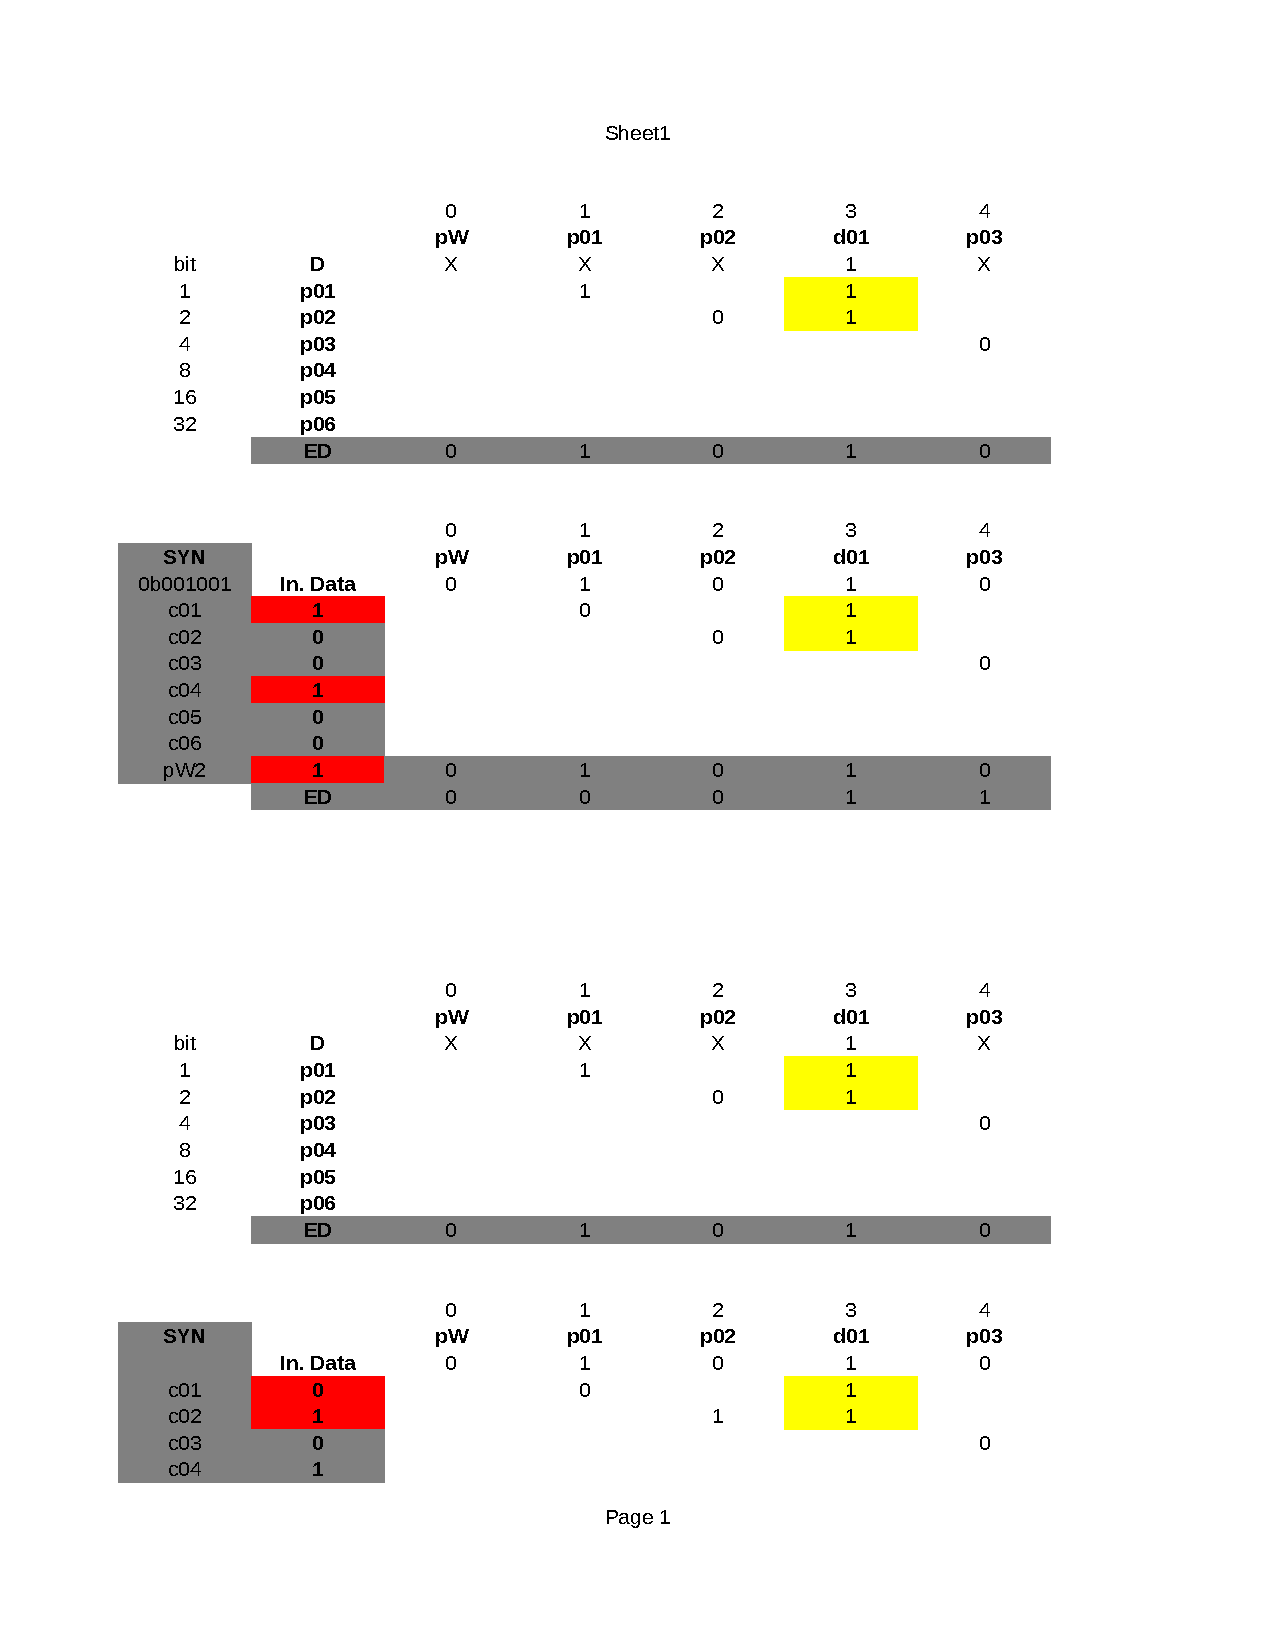
\includepdf[pages=-]{code/rtos_hamming_code.pdf}
	\pagebreak
\end{appendices}


\vspace{1cm}
\hrule
\vspace{0.5cm}


%---------------------------------------------------------------------------
\end{document}
-
